\documentclass[
    %uninadraft,
    %colorlinks, 
    blacklinks,
    %palatino,
    libertine,
    %mathpazo,
    %tgschola,
    %tgscholamathpazo,
    %alegreya
]{uninathesis}

%\AtBeginDocument{\addtocontents{toc}{\protect\thispagestyle{empty}}} %remove page number from toc

\usepackage[italian]{babel}
\addto\captionsenglish{% Replace "english" with the language you use
  \renewcommand{\contentsname}%
    {\sffamily Contents}%
}

% Math
\RequirePackage{mathtools}
\RequirePackage{mathrsfs} %need this for mathscr
\let\openbox\relax
\RequirePackage{amsthm}
\RequirePackage{stmaryrd} %for \llbracket

\usepackage{mdframed}
\theoremstyle{plain}
\newmdtheoremenv[linewidth=1pt,nobreak=true,innertopmargin=0pt,backgroundcolor=yellow!10, skipabove=1em]{theorem}{Teorema}
\newmdtheoremenv[linewidth=1pt,nobreak=true,innertopmargin=0pt,skipabove=1em]{lemma}{Lemma}

\newtheorem{property}{Proprietà}
\theoremstyle{definition}
\newtheorem{definition}{Definizione}
\newtheorem{example}{Esempio}
\newtheorem*{remark}{Nota bene}

% Tikz - may be removed if unneeded
\RequirePackage{tikz}
\usepackage{pgfplots}
\pgfplotsset{compat=1.16}
\usetikzlibrary{positioning,automata,calc,fit,shapes,backgrounds,arrows.meta}
\usepackage{makecell}

% Miscellanea Packages
\RequirePackage[utf8]{inputenc}
\usepackage{ marvosym } %/Lightning
%\usepackage{ stmaryrd } %/lightning
%\usepackage[htt]{hyphenat}
\usepackage{subcaption} %subfigures
\usepackage{pgf-umlcd}
\usepackage{wrapfig}
\usepackage{csvsimple}
\renewcommand{\umldrawcolor}{black}
\makeatletter
\renewcommand{\ALG@name}{Algoritmo}
\algnewcommand\algorithmicswitch{\textbf{switch}}
\algnewcommand\algorithmiccase{\textbf{case}}
% New "environments"
\algdef{SE}[SWITCH]{Switch}{EndSwitch}[1]{\algorithmicswitch\ #1\ \algorithmicdo}{\algorithmicend\ \algorithmicswitch}%
\algdef{SE}[CASE]{Case}{EndCase}[1]{\algorithmiccase\ #1}{\algorithmicend\ \algorithmiccase}%
\algtext*{EndSwitch}%
\algtext*{EndCase}%
\makeatother
\raggedbottom

\usepackage{import}
\usepackage{pdfpages}
\usepackage{transparent}

\newcommand{\incfig}[2][1]{%
    \def\svgwidth{#1\columnwidth}
    \import{./figures/}{#2.pdf_tex}
}

\pdfsuppresswarningpagegroup=1

% Bibliography
\RequirePackage{csquotes}
\RequirePackage[sorting=none,maxbibnames=4]{biblatex} %dashed=false to remove dashes on repeated authors.
\bibliography{bib/bibliography.bib} %bib database(s)

% Front page (package uninafrontespizio)
\Universita{Università degli Studi di Napoli Federico II}
\Facolta{Scuola Politecnica e delle Scienze di Base}
\Dipartimento{Dipartimento di Ingegneria Elettrica e Tecnologie dell'Informazione}
\CorsoDiLaurea{Corso di Laurea Triennale in Informatica}
%\Materia{Verifica di Sistemi}
\AnnoAccademico{2022--2023}
\Titolo{Implementazione di una procedura di decisione per il frammento guarded in Vampire}
\Relatore{Prof. Fabio \textsc{Mogavero}\\Prof. Massimo \textsc{Benerecetti}}
\RelatoreLabel{Relatori}
\Candidato{Francesco \textsc{Scarfato}}
\Matricola{N86/3769}
\Logo{logo-federico-II.pdf}
\LogoWidth{3.5cm}
\LogoPosition{below-uni}

%custom hyphenation
\hyphenation{ERTMS/ETCS}

\usepackage[title,titletoc]{appendix}

\begin{document}
    \pagestyle{empty}
    \frontmatter
    \makefrontespizio~\clearpage
    \makefrontespizioalt~\clearpage

    %\pagestyle{backmatter}
    %\input{_chapters/0-abstract.tex}
    
    \clearpage
    \tableofcontents

    \mainmatter

    \pagestyle{introduction}
\chapter*{Introduzione}
\addcontentsline{toc}{chapter}{Introduzione}
Un \emph{theorem prover} è un importante strumento che permette di verificare formalmente 
sistemi software e hardware, strettamente collegato ai campi della logica e della matematica.
I \emph{theorem prover} sono degli strumenti \emph{general purpose} che puntano a risolvere il maggior numero di problemi nel modo più veloce 
ed efficiente possibile. Per migliorare questi sistemi, la ricerca si sta muovendo verso la definizione di 
procedure di decisione per problemi decidibili. Una procedura di decisione è un algoritmo che verifica 
la soddisfacibilità di un problema e arriva sempre a una terminazione. Nella logica del primo ordine, un sottoinsieme di problemi decidibili è detto 
frammento. La ricerca di queste procedure di decisione è rilevante poiché, in alcuni casi, questi approcci possono risultare 
più efficienti di una strategia general purpose. L'ideale sarebbe inglobare queste procedure di decisione nei 
theorem prover, quando è possibile, e utilizzarle nel caso in cui un problema appartenga a un determinato frammento.

In questa tesi viene presentata un'implementazione di una procedura di decisione per il frammento \emph{guarded} su   
\textsc{Vampire}, uno degli \emph{automated theorem prover}, per la risoluzione di 
problemi di logica del primo ordine, più conosciuti ed efficienti in circolazione. Nella prima parte vengono introdotte le caratteristiche base
più importanti di \textsc{Vampire} e del frammento \emph{guarded}. Nella seconda parte viene descritta 
l'implementazione sperimentale della procedura di decisione per questo particolare frammento. Infine, viene presentata un'analisi basata sul 
confronto tra il software originario e la versione estesa con la procedura di decisione. 


    \newpage\pagestyle{main}
    \chapter{Panoramica su Vampire}
In questo capitolo viene presentato il theorem prover \textsc{Vampire}, la sua architettura e alcune
delle caratteristiche più importanti.

\section{Cos'è \textsc{Vampire}}
\textsc{Vampire} è un sistema che permette di provare la validità di teoremi (matematici e non) di logica del primo ordine. 
Il linguaggio di programmazione usato è C++ e la prima versione è stata sviluppata principalmente 
da Andrei Voronkov e Krystof Hoder tra il 1993 e il 1995 nell'Università di Manchester. Dopo il 1995, 
il progetto è stato sospeso e viene ripreso nel 1998. Dal '98 vengono implementate numerose versioni e, 
ancora oggi, proseguono gli sviluppi. \textsc{Vampire} ha vinto circa 45 titoli in diverse divisioni 
della CASC (CADE ATP System Competition) che è il campionato mondiale per gli ATP (Automated Theorem Prover).
Ecco alcune delle principali caratteristiche del sistema:
\begin{itemize}
    \item è molto veloce
    \item è portabile sulle piattaforme più comuni
    \item è semplice da usare
    \item ha strategie di ricerca con risorse limitate
    \item supporta numerose sintassi in input
    \item i vari tentativi per provare il problema possono essere parallelizzati su più processori
    \item può produrre, in base alle opzioni selezionate, output molto dettagliati 
\end{itemize}
\section{Architettura di \textsc{Vampire}}
\textsc{Vampire} ha un'architettura complessa ma, analizzandola da un alto livello, è possibile riconoscere tre moduli 
principali:
\begin{enumerate}
    \item \emph{parser}
    \item \emph{preprocessor}
    \item \emph{kernel}
\end{enumerate}
\begin{figure}[H]
    \incfig{architettura}
\end{figure}


\subsection{Parser}
Il \emph{parser} è un modulo adibito al parsing del problema. Il problema viene letto da un file e viene incapsulato in una classe.
Nel caso di un problema di logica del primo ordine con sintassi TPTP, allora viene diviso in più unità.
Ogni unità è una formula o una clausola a cui viene assegnato uno specifico tag in base al tipo (ipotesi, assioma, congettura, teorema, \dots).
Nel codice sorgente sono presenti le classi \verb|Problem|, \verb|Unit|, \verb|Formula|, \verb|Clause| e sono in relazione tra loro come mostrato nella figura \ref{fig:relazioni-classi}.
Oltre alle rappresentate \verb|NegatedFormula| e \verb|QuantifiedFormula|, sono presenti altre classi che ereditano \verb|Formula| come
\verb|AtomicFormula|, \verb|JunctionFormula|, \verb|BinaryFormula|, \dots
\begin{remark}
    Un' unità può essere una formula o una clausola ma non entrambe. La distinzione viene effettuata sulla base dell'
    attributo \emph{kind} che è un' enumerazione.
\end{remark}
\vspace{.3cm}
\begin{figure}[H]
    \begin{tikzpicture}
        \begin{class}{Problem}{-5,0}
            \attribute{- units : UnitList*}
        \end{class}
        \begin{class}{Unit}{-5,-2}
            \attribute{- kind : enum}
            \operation{+ getFormula()}
            \operation{+ asClause()}
        \end{class}
        \begin{class}{Formula}{-10,-5}
        \end{class}
        \begin{class}{Clause}{0,-5}
        \end{class}
        \begin{class}{QuantifiedFormula}{-10,-8}
            \inherit{Formula}
        \end{class}
        \begin{class}{NegatedFormula}{-4,-8}
            \inherit{Formula}
        \end{class}
    
        \unidirectionalAssociation{Problem}{}{}{Unit}
        \unidirectionalAssociation{Unit}{}{}{Formula}
        \unidirectionalAssociation{Unit}{}{}{Clause}
    \end{tikzpicture}
    \caption{Relazioni tra le classi}\label{fig:relazioni-classi}
\end{figure}
\subsection{Preprocessor}
Il \emph{\emph{preprocessor}} è un modulo che processa il problema in modo che sia trattabile dal \emph{kernel} in fase di risoluzione.
Per questo modulo è possibile abilitare numerose opzioni, inoltre vengono eseguite molte semplificazioni in modo da rendere il sistema il 
più veloce possibile. Di seguito sono descritti solo i passaggi fondamentali: 
\begin{description}
    \item[I step] \emph{Rectify} $\longrightarrow$ Il \emph{preprocessor} verifica se una formula ha variabili libere. Se la formula è aperta, 
    allora genera dei quantificatori per vincolare le variabili libere. Inoltre, verifica che per ogni variabile $x$ ci sia una sola occorrenza di $\exists x$ o $\forall x$. 
    \item[II step] \emph{Simplify} $\longrightarrow$ Il \emph{preprocessor} verifica se una formula contiene $\top$ o $\bot$. Nel caso la formula contenesse uno dei due, allora
    viene semplificata.
    \item[III step] \emph{Flatten} $\longrightarrow$ Il \emph{preprocessor} trasforma le formule in modo da renderle uniformi. Questo è solo uno step di formattazione che verrà eseguito più volte nel corso del preprocessing.
    \item[IV step] \emph{Unused definitions and pure predicate removal} $\longrightarrow$ Il \emph{preprocessor} rimuove i predicati e le definizioni delle funzioni che non vengono usati.
    \item[V step] \emph{ENNF} $\longrightarrow$ Il \emph{preprocessor} trasforma le formula in modo da ottenerle in \emph{extended negative normal form}.
    \begin{definition}
        Una formula è in \emph{extended negation normal form} se non contiene $\rightarrow$ e tutte le $\neg$ sono spostate, il più possibile, verso l'interno.  
    \end{definition}
    \item[VI step] \emph{Naming} $\longrightarrow$ Il \emph{preprocessor} definisce un nuovo predicato $p$ che viene usato come nome di una sotto-formula. 
    Questa tecnica viene utilizzata per evitare di generare un numero esponenziale di clausole nei prossimi passaggi di preprocessing.
    \begin{definition}
        Sia $\varphi|_\pi$ sotto-formula di $\varphi$ in posizione $\pi$ con variabili libere $\bar{x}$, allora si sostituisce $\varphi|_\pi$ con $p(\bar{x})$
        nuovo predicato e viene aggiunta la definizione $\text{def}(\varphi,\pi,p)$ tale che
        \[\text{def}(\varphi,\pi,p)=\begin{cases}
            \forall \bar{x} (p(\bar{x})\rightarrow \varphi|_\pi) & \text{se pol}(\varphi,\pi)=1\\
            \forall \bar{x} (\varphi|_\pi\rightarrow p(\bar{x})) & \text{se pol}(\varphi,\pi)=-1\\
            \forall \bar{x} (p(\bar{x})\leftrightarrow \varphi|_\pi) & \text{se pol}(\varphi,\pi)=0\\
        \end{cases}\]
        in cui $\text{pol}(\varphi,\pi)$ indica la polarità della sotto-formula di $\varphi$ in posizione $\pi$. $\text{pol}(\varphi,\pi)=0$ si verifica quando il simbolo di livello superiore di $\varphi|_\pi$ è 
        $\leftrightarrow$ o $\otimes$.   
    \end{definition}
    \begin{remark}
        Questa tecnica viene adottata solo se il numero di clausole generate supera una certa soglia. Infatti, in 
        \textsc{Vampire}, nella classe \verb|Naming|, è presente un attributo \emph{threshold} che indica proprio questo limite.
    \end{remark}
    \item[VII step] \emph{NNF} $\longrightarrow$ Il \emph{preprocessor} trasforma le formula in modo da ottenerle in \emph{negation normal form}.
    \begin{definition}
        Una formula è in \emph{negation normal form} se non contiene $\rightarrow,\leftrightarrow,\otimes$ e tutte le $\neg$ sono spostate, il più possibile, verso l'interno.
    \end{definition}
    \item[VIII step] \emph{Skolemization} $\longrightarrow$ Il \emph{preprocessor} applica la tecnica di skolemizzazione per eliminare i $\exists$ dalle formule.
    \begin{definition}
        Sia $F=\exists x\mid\varphi(y_1,\dots,y_n,x)$ formula in negation normal form allora la skolemizzazione si ottiene tramite la seguente sostituzione:
        \[F=\exists x\mid\varphi(y_1,\dots,y_n,x)\Rightarrow F'=\varphi(y_1,\dots,y_n,x)\{x \mapsto sk(y_1,\dots,y_n)\}\]
        in cui $\{x \mapsto sk(y_1,\dots,y_n)\}$ indica che $x$, la variabile precedentemente vincolata dal quantificatore esistenziale nella formula $F$, 
        è sostituita da una nuova funzione $sk(y_1,\dots,y_n)$, detta di Skolem, nella formula $F'$.
    \end{definition}
    \item[IX step] \emph{Clausification} $\longrightarrow$ Il \emph{preprocessor} applica la clausificazione su tutte le formule in modo da ottenere 
    un insieme di clausole.
    \begin{definition}
        La clausificazione è il risultato di:
        \begin{enumerate}
            \item $\forall x\mid\varphi(y_1,\dots,y_n,x)\Rightarrow\varphi(y_1,\dots,y_n,x)\{x \mapsto X\}$  in cui $X$ è una variabile designata che non occorre in $\varphi$
            \item Se una formula $F=\varphi'\land\varphi''$ allora viene spezzata in due unità diverse 
            $F'=\varphi'$ e $F''=\varphi''$
        \end{enumerate}
    \end{definition}  
\end{description} 
Alla fine di questi step, l'insieme di clausole risultanti è pronto per essere passato all'algoritmo di \emph{resolution}.
\subsection{Kernel}
Il \emph{kernel} è il sotto-sistema adibito alla risoluzione del problema. Per raggiungere questo obiettivo, 
viene implementato un algoritmo di saturazione che permette di trovare una confutazione all'insieme di clausole.
Questo è possibile tramite la saturazione dell'insieme con tutte le possibili inferenze presenti nel calcolo. 
\textsc{Vampire} possiede numerose inferenze ma è possibile sceglierne un sottoinsieme e definire un sistema 
d'inferenze per la logica del primo ordine.

Formalmente, per definire un sistema d'inferenze bisogna prima definire un \emph{simplification ordering} e una funzione di selezione.
\begin{definition}
    Un ordinamento $\succ$ sui termini è detto \emph{simplification ordering} se rispetta le seguenti condizioni:
    \begin{enumerate}
        \item $\succ$ è ben formato ovvero $\nexists t_0,t_1, \dots \text{sequenza infinita tale che } t_0 \succ t_1 \succ \dots$
        \item $\succ$ è monotona ovvero $l \succ r \rightarrow s(l)\succ s(r)$ per tutti i termini $s,l,r$
        \item $\succ$ è stabile per la sostituzione ovvero $l \succ r \rightarrow l\theta \succ r\theta$
        \item $\succ$ ha la \emph{subterm property} ovvero se $r$ sottotermine di $l$ e $l\neq r$ allora $l\succ r$   
    \end{enumerate}
\end{definition}
Questa definizione è estendibile agli atomi, ai letterali e alle clausole.
\begin{definition}
    Una funzione di selezione seleziona un sottoinsieme non vuoto di letterali in ogni clausola non vuota. In $\underline{L}\lor R$ \underline{L} indica il letterale selezionato.
\end{definition}
Il sistema di inferenze che viene definito di seguito è detto \emph{superposition inference system}.
\begin{definition}
    Il \emph{superposition inference system} è un sistema di inferenze composto dalle seguenti regole
    \begin{itemize}
        \item \textbf{Resolution}
        \begin{equation}
            \begin{gathered}
                \underline{\underline{A} \lor C_1 \quad\underline{\lnot A'}\lor C_2}\\
                (C_1 \lor C_2)\theta
            \end{gathered}
        \end{equation}
        in cui $\theta$ è l'unificatore più generale di $A$ e $A'$.
        \item \textbf{Factoring}
        \begin{equation}
            \begin{gathered}
                \underline{\underline{A} \lor \underline{A'} \lor C}\\
                (A \lor C)\theta
            \end{gathered}
        \end{equation}
        in cui $\theta$ è l'unificatore più generale di $A$ e $A'$.
        \item \textbf{Superposition}
        \begin{equation}
            \begin{gathered}
                \underline{\underline{l=r} \lor C_1 \quad \underline{L[s]}\lor C_2} \quad \underline{\underline{l=r} \lor C_1 \quad \underline{t[s]=t'}\lor C_2} \quad \underline{\underline{l=r} \lor C_1 \quad \underline{t[s]\neq t'}\lor C_2}\\
                (L[r] \lor C_1 \lor C_2)\theta \qquad (t[r]=t' \lor C_1 \lor C_2)\theta \qquad (t[r]\neq t' \lor C_1 \lor C_2)\theta
            \end{gathered}
        \end{equation}
        in cui $\theta$ è l'unificatore più generale di $l$ e $s$, $s$ non è una variabile, 
        $r\theta\prec l\theta$, solo nella prima regola $L[s]$ non è un \emph{equality literal}\footnote{Un \emph{equality literal} è una clausola 
        con un singolo letterale in cui è presente un =},
        \item \textbf{Equality resolution}
        \begin{equation}
            \begin{gathered}
                \underline{\underline{s\neq t} \lor C}\\
                C\theta
            \end{gathered}
        \end{equation}
        in cui $\theta$ è l'unificatore più generale di $s$ e $t$.
        \item \textbf{Equality factoring}
        \begin{equation}
            \begin{gathered}
                \underline{\underline{s=t} \lor \underline{s'=t'}\lor C}\\
                (s=t \lor t\neq t' \lor C)\theta
            \end{gathered}
        \end{equation}
        in cui $\theta$ è l'unificatore più generale di $s$ e $t$, $t\theta \prec s\theta$ e $t'\theta\prec t\theta$.
    \end{itemize}
\end{definition}
Se la funzione di selezione seleziona sia letterali negativi sia tutti i letterali massimali, allora è possibile enunciare la seguente proprietà: 
\begin{property}\label{sup}
    Il superposition inference system è sound e completo.
\end{property}
Una volta definito un sistema di inferenze, è possibile formalizzare il concetto di saturazione espresso precedentemente.
\begin{definition}
    Un insieme di clausole $S$ è detto saturato rispetto al sistema di inferenze $\phi$ se, 
    per ogni inferenza in $\phi$ con le premesse in $S$, la conclusione dell'inferenza appartiene sempre
    a $S$. 
\end{definition}
Grazie alla proprietà \ref{sup}, si ottiene questa importante proprietà:
\begin{property}
    Un insieme di clausole è \textbf{insoddisfacibile} se, e solo se, il più piccolo insieme di clausole contenente $S$, saturato 
    rispetto al superposition inference system, contiene anche la clausola vuota $\square$
\end{property}

Per rendere efficiente l'algoritmo di saturazione, oltre a queste regole, vengono introdotte
regole di semplificazione per eliminare ridondanze e semplificare le inferenze. Alcune di queste regole sono: \emph{demodulation},
\emph{branch demodulation} e \emph{subsumption resolution}. 

In generale, un algoritmo di saturazione è composto dalle seguenti fasi:
\begin{enumerate}
    \item Viene inizializzato un insieme $S$ in cui vengono memorizzate le clausole
    \item Viene selezionata un'inferenza che può essere applicata a delle clausole presenti in $S$
    \item Nel caso fosse generato un risultato, allora viene aggiunto a $S$
    \item Se viene trovata una clausola vuota $\square$, allora il problema è insoddisfacibile
\end{enumerate}
Se un'inferenza genera una clausola, allora è detta generatrice. Le inferenze generatrici 
sono strettamente collegate alle regole di semplificazioni.
\textsc{Vampire} implementa tre tipi di algoritmi di saturazione: \emph{limited resource strategy}(lrs), \emph{otter} e \emph{discount}.
Tutti fanno parte della famiglia dei \emph{given clause algorithm}.
\begin{algorithm}
    \caption{Given clause algorithm}
    \begin{algorithmic}[1]
        \State \textbf{var} active,passive : sets of clause 
        \State \textbf{var} current,new : clause
        \State active = $\emptyset$
        \State passive = set of input clauses
        \While{passive $\neq \emptyset$}
            \State current = \emph{select}(passive)
            \State passive = passive $\setminus$ $\{\text{current}\}$
            \State active = active $\cup$ $\{\text{current}\}$
            \State new = \emph{infer}(current,active)
            \If{new is $\square$}
                \State \underline{\textbf{return} provable}
            \EndIf
            \State passive = passive $\cup$ $\{\text{new}\}$ 
        \EndWhile
        \State \underline{\textbf{return} unprovable}
    \end{algorithmic}
\end{algorithm}
\cite{kovacs2013first,riazanov2002design,reger2016new}
    \clearpage
    \let\cleardoublepage\relax
\chapter{Frammento Guarded}
Il frammento \emph{guarded} è un frammento della logica del primo ordine introdotto da Hajnal Andréka,
István Nèmeti e Johan van Benthem. L'importanza è dovuta alla possibilità  di tradurre 
molte logiche modali, con significative proprietà computazionali e logiche, in formule del primo ordine 
appartenenti al frammento \emph{guarded}. \'E stato provato che questo frammento (con uguaglianza e non) 
è decidibile in \textsc{2-EXPTIME}. 

Sono state proposte numerose generalizzazioni di questo frammento in quanto
alcune logiche modali importanti (come quella temporale) non possono essere tradotte. La generalizzazione 
piu datata è il frammento \emph{loosely guarded} che ha dei vincoli meno stringenti sulla definizione di guardia.
L'implementazione della procedura di decisione in questa tesi riguarda il frammento \emph{guarded} senza uguaglianza \cite{de2003deciding}.
\begin{definition}
    Il frammento \emph{guarded} è ricorsivamente definito come i seguenti sottoinsiemi di logica del primo ordine senza
    uguaglianza e simboli di funzione:
    \begin{enumerate}
        \item $\top,\bot\in$ GF.
        \item Se $a$ è una formula atomica, allora $a\in$ GF.
        \item GF è chiuso rispetto a $\lnot, \land,
        \lor, \rightarrow, \leftrightarrow$.
        \item Sia $A\in$ GF, $a$ formula atomica tale che ogni variabile libera di $A$ occorra almeno una volta negli argomenti 
        di $a$. Allora 
        \begin{itemize}
            \item $\forall\bar{x}(a \rightarrow A)\in$ GF,
            \item $\exists\bar{x}(a \land A)\in$ GF,
            \item $\forall\bar{x}(a \lor A)\in$ GF (negazione della precedente)
        \end{itemize}
        con la formula atomica $a$ definita \textbf{guardia}.
    \end{enumerate}
\end{definition}
Dopo aver delineato quando una formula del primo ordine appartiene al frammento \emph{guarded}, di seguito viene 
definito quando una clausola è \emph{guarded}.
\begin{definition}
    Una clausola $c$ è \emph{guarded} se soddisfa le seguenti condizioni:
    \begin{enumerate}
        \item Ogni termine funzionale non \emph{ground} in $c$ contiene tutte le variabili di $c$.
        \item Se $c$ è non ground allora c'è un letterale negativo $\lnot A$ in $c$ che contiene tutte le variabili di $c$ ma 
        non contiene termini funzionali non \emph{ground}.

        Il letterale negativo $\lnot A$ è definito \textbf{guardia}.
    \end{enumerate}
    Se la clausola $c$ è \emph{ground}, allora è \emph{guarded}.
\end{definition}
\begin{definition}
    Una insieme formato da clausole \emph{guarded} è anch'esso \emph{guarded}
\end{definition}
\section{Preprocessing}
Come menzionato nel precedente capitolo \ref{sec-prepro}, il problema viene pre-processato per ottenere un insieme di clausole 
da sottomettere all'algoritmo di risoluzione. Le operazioni di \emph{preprocessing} sono le seguenti:
\begin{enumerate}
    \item \emph{Negation normal form} 
    \item $\text{\emph{Struct}}_\forall$
    \item \emph{Skolemization}
    \item \emph{Clausification}
\end{enumerate} 
L'unica operazione non ancora definita è $\text{\emph{Struct}}_\forall$.
\begin{definition}\label{struct-def}
    $\text{\emph{Struct}}_\forall$ è una trasformazione strutturale che è ottenuta da:
    \begin{enumerate}
        \item la sostituzione delle sotto-formule $\forall\bar{x}(a \rightarrow A)$, $\forall\bar{x}(a \lor A)$ che hanno 
        $\bar{y}$ variabili libere, con un nuovo nome $\alpha(\bar{y})$
        \item l'aggiunta della formula $\forall\bar{x}\bar{y}(\lnot a \lor \lnot\alpha \lor A)$
    \end{enumerate}
\end{definition}
Queste operazioni, oltre a generare un insieme di clausole, preservano l'appartenenza delle formule al frammento \emph{guarded}.
\begin{theorem}
    Sia $F\in$ GF allora 
    \begin{enumerate}
        \item $F'=\text{NNF}(F) \in$ GF,
        \item $F''=\text{\emph{Struct}}_\forall(F') \in$ GF,
        \item applicando skolemization e clausification a $F''$ si ottiene un insieme di clausole guarded.
    \end{enumerate}
\end{theorem}
Il teorema è dimostrato nello studio di \citeauthor{de2003deciding} in \cite{de2003deciding}.
\section{Resolution}
La procedure di decisione per il frammento \emph{guarded} necessita della definizione di una nuova regola di risoluzione.
Prima di definire tale regola, è necessario stabilire: un ordinamento e dei parametri secondo cui ordinare.
\begin{definition}\label{var-def}
    La \emph{Vardepth} di un termine/atomo $A$ è definita ricorsivamente come segue:
    \[\text{\emph{Vardepth}}(A) = 
    \begin{cases}
        -1 & \text{se $A$ è ground}\\
        0 & \text{se $A$ è una variabile}\\
        \max\{1+\text{\emph{Vardepth}}(t_1), \dots, 1+\text{\emph{Vardepth}}(t_n)\} & \text{se }A=f(t_1,\dots,t_n)
    \end{cases}\]
\end{definition}
\begin{definition}
    La \emph{Vardepth} di un letterale equivale alla \emph{Vardepth} di un atomo.
\end{definition}
\begin{definition}
    La \emph{Vardepth} di una clausola $c$ equivale alla \emph{Vardepth} massimale di un letterale in $c$. 
\end{definition}
\begin{definition}
    Sia $A$ atomo, letterale o clausola, allora \emph{Var}$(A)$ è definito come l'insieme delle 
    variabili che occorrono in $A$.
\end{definition}
Una volta definiti questi due parametri \emph{Vardepth} e \emph{Var}, è possibile definire l'ordinamento.
\begin{definition}\label{ord-def}
    Definiamo l'ordinamento $\prec$ sui letterali $A,B$ come segue:
    \[A\prec B \quad\text{se}\quad(\text{\emph{Vardepth}}(A)<\text{\emph{Vardepth}}(B)) \lor (\text{\emph{Var}}(A)\subset\text{\emph{Var}}(B))\]
\end{definition}
Ora è possibile introdurre la nuova regola di risoluzione definita \emph{ordered resolution rule}.
\begin{definition}
    Sia $\prec$ ordinamento sui letterali, $\{A_1\}\cup R_1$ e $\{\lnot A_2\}\cup R_2$ clausole allora se:
    \begin{enumerate}
        \item $\{A_1\}\cup R_1$ e $\{\lnot A_2\}\cup R_2$ non hanno variabili in comune,
        \item $A_1$ deve essere massimale in $R_1$ ovvero $\nexists A\in R_1 : (A_1 \prec A)$,
        \item $A_2$ deve essere massimale in $R_2$ ovvero $\nexists A\in R_2 : (A_2 \prec A)$,
        \item $A_1$ e $A_2$ hanno un unificatore più generale (\emph{mgu}) $\theta$,
    \end{enumerate}
    allora $R_1\theta \cup R_2\theta$ è chiamato $\prec$-\emph{ordered resolvent} di $\{A_1\}\cup R_1$ e $\{\lnot A_2\}\cup R_2$.
    \begin{equation}
        \begin{gathered}
            \underline{\{\underline{A_1}\} \lor R_1 \quad\{\underline{\lnot A_2}\}\lor R_2}\\
            (R_1 \lor R_2)\theta
        \end{gathered}
    \end{equation}
\end{definition}
Questa regola è una \emph{resolution rule} (\ref{res-eq}) ristretta da un'ordinamento $\prec$. \'E possibile
definire anche una  \emph{factorization rule} (\ref{fact-eq}) ristretta.
\begin{definition}
    Sia $\prec$ ordinamento sui letterali, $\{A_1,A_2\}\cup R$ clausola allora se:
    \begin{enumerate}
        \item $A_1$ deve essere massimale in $R$ ovvero $\nexists A\in R : (A_1 \prec A)$,
        \item $A_1$ e $A_2$ hanno un unificatore più generale (\emph{mgu}) $\theta$,
    \end{enumerate}
    allora $\{A_1\theta\}\cup R\theta$ è chiamato $\prec$-\emph{ordered factor} di $\{A_1,A_2\}\cup R$.
    \begin{equation}
        \begin{gathered}
            \underline{\{\underline{A_1} \lor \underline{A_2}\} \lor R}\\
            (A_1 \lor R)\theta
        \end{gathered}
    \end{equation}
\end{definition}
Nell'algoritmo di risoluzione è necessaria una \emph{resolution rule} ristretta dall'ordinamento $\prec$ poiché preserva 
la proprietà degli $\prec$-\emph{ordered resolvent} di essere \emph{guarded}. Invece la \emph{factorization rule}
\textbf{preserva la proprietà delle clausole di essere \emph{guarded} anche senza applicare una restrizione}.
Tutto questo viene provato dal seguente teorema per la cui dimostrazione si rimanda a \cite{de2003deciding}:
\begin{theorem}
    \begin{enumerate}
        \item Se $c_1$ e $c_2$ sono clausole \emph{guarded} allora $c$ $\prec$-\emph{ordered resolvent} di $c_1$ e $c_2$ è
        \emph{guarded}
        \item Se $c_1$ è una clausola \emph{guarded} allora $c$ \emph{factor} di $c_1$ è \emph{guarded}
    \end{enumerate}
\end{theorem}
Un algoritmo di risoluzione, per essere definito procedura di decisione, deve terminare ed essere completo.

L'algoritmo con la $\prec$-\emph{ordered resolution rule} e la \emph{factorization rule} termina perché, grazie alla restrizione
sulla \emph{resolution rule}, è possibile derivare solo un insieme finito di clausole da un insieme finito di clausole \emph{guarded}. 
\begin{lemma}
    Sia $C$ un insieme finito di clausole \emph{guarded}. Se $\bar{C}$ è l'insieme generato da $C$ tramite 
    la $\prec$-\emph{ordered resolution rule} e la \emph{factorization rule}, allora $\bar{C}$ ha dimensione finita.
\end{lemma}
La dimostrazione di questo lemma è possibile poiché il numero di variabili e la \emph{Vardepth} sono limitati superiormente \cite{de2003deciding}. 

\begin{definition}
    Un algoritmo di risoluzione è completo per una logica se riesce a risolvere ogni problema appartenente
    a quella logica. 
\end{definition}
Nello studio di \citeauthor{de2003deciding} è presentata la dimostrazione della completezza per la procedura di decisione \cite{de2003deciding}.
    \clearpage
    \chapter{Implementazione della procedura}\label{second-c}
Come descritto nel precedente capitolo, la procedura di decisione per problemi
appartenenti al frammento \emph{guarded} è formata da una fase di \emph{preprocessing} e 
una fase di risoluzione tramite $\prec$-\emph{ordered resolution} e \emph{factorization}. 
\begin{figure}[H]
    \incfig{architettura-2}
    \caption{Struttura di \textsc{Vampire} prima delle modifiche}
\end{figure}
L'idea per l'implementazione della procedura è:
\begin{enumerate}
    \item costruire un nuovo \emph{preprocessor} che trasformi le formule \emph{guarded} in clausole e sostituirlo nel sistema
    \item implementare una nuova inferenza ($\prec$\emph{-ordered resolution}) e ``iniettarla" nell'algoritmo di saturazione
    \item eliminare tutte le inferenze non necessarie dall'algoritmo di saturazione 
\end{enumerate}
\begin{figure}[H]
    \incfig{architettura-3}
    \caption{Struttura di \textsc{Vampire} dopo le modifiche}
\end{figure}
\section{Preprocessing}
Per quanto riguarda la fase di \emph{preprocessing}, è stato sviluppato un \emph{preprocessor} per trattare problemi 
appartenenti al frammento \emph{guarded}. Questa componente è stata implementata seguendo l'architettura 
del \emph{preprocessor} predefinito di \textsc{Vampire}.
\begin{algorithm}
    \caption{Preprocessing}
    \begin{algorithmic}
        \State \textbf{var} problem : sets of guarded formula
        \State \textbf{var} result : sets of guarded clause 
        \State problem = \emph{NNF}(problem)
        \State problem = \emph{flatten}(problem)
        \State problem =$\text{\emph{Struct}}_\forall$(problem)
        \State problem = \emph{skolemize}(problem)
        \State result = \emph{clausify}(problem)
        \State \emph{computeVarDepth}(result)
        \State \underline{\textbf{return} result}
    \end{algorithmic}
\end{algorithm}

\emph{NNF, flatten, skolemize} e \emph{clausify} (descritte in \ref{sec-prepro}) sono le funzioni di 
\textsc{Vampire} che vengono sfruttate per la trasformazione del problema.
Invece le funzioni $\text{\emph{Struct}}_\forall$ e \emph{computeVarDepth} vengono implementate ex-novo in quanto non presenti 
nel sistema. 

$\text{\emph{Struct}}_\forall$ è una funzione ricorsiva che sfrutta la struttura ad albero delle formule.
\begin{figure}[H]
    \incfig{tree}
    \caption{Struttura ad albero della formula}
\end{figure}
L'intero albero sintattico della formula viene visitato tramite una visita post-order. Durante la visita, l'algoritmo 
controlla se nell'intero albero sono presenti formule del tipo $\forall \bar{x}(a \lor A)$ con almeno una variabile libera.
Nel caso venga trovata una formula in questa forma, viene applicata la trasformazione strutturale 
$\text{\emph{Struct}}_\forall$.

\begin{algorithm}[H]
    \caption{Visita post-order}
    \begin{algorithmic}
        \Function{\textsc{PostOrderVisit}}{input : formula}
            \Case{connective \textbf{of} input}
                \Switch{$\top,\bot$, Literal}
                    \State \underline{\textbf{return} input}
                \EndSwitch
                \Switch{$\lnot,\exists$}
                    \State \underline{\textbf{return} \textsc{PostOrderVisit}(subformula \textbf{of} input)}
                \EndSwitch
                \Switch{$\rightarrow,\leftrightarrow$}
                    \State \textbf{var} left, right : formula
                    \State left = \textsc{PostOrderVisit}(left subformula \textbf{of} input)
                    \State right = \textsc{PostOrderVisit}(right subformula \textbf{of} input) 
                    \State \underline{\textbf{return} input}
                \EndSwitch
                \Switch{$\land,\lor$}
                    \ForAll{subformula \textbf{in} input}
                        \State subformula = \textsc{PostOrderVisit}(subformula)
                    \EndFor
                    \State \underline{\textbf{return} input} 
                \EndSwitch
                \Switch{$\forall$}
                    \State \textbf{var} subformula : formula
                    \State subformula = \textsc{PostOrderVisit}(subformula \textbf{of} input)
                    \If{(connective \textbf{of} subformula \textbf{is} $\lor$) $\land$ (\emph{hasFreeVar}(input))}
                        \State  input=$\text{\emph{Struct}}_\forall$(input)
                    \EndIf
                    \State \underline{\textbf{return} input}
                \EndSwitch  
            \EndCase
        \EndFunction
    \end{algorithmic}
\end{algorithm}
Per l'implementazione della trasformazione strutturale, si segue la definizione \ref{struct-def}.
\begin{algorithm}[H]
    \caption{$\text{\emph{Struct}}_\forall$}
    \begin{algorithmic}
        \Function{\textsc{$\text{\emph{Struct}}_\forall$}}{input : formula}
        \State \textbf{var} new, $\alpha$ : formula
        \State \textbf{var} $\bar{y}$ : sets of free variables 
        \State $\bar{y} =$ \emph{saveFreeVariable}(input)
        \State $\alpha =$ \emph{createNewLiteral}($\bar{y}$)
        \State new = \emph{generateNewFormula}($alpha$,input)
        \State \emph{addFormulaToUnits}(new)
        \State input = $\alpha$
        \State \underline{\textbf{return} input}
        \EndFunction
    \end{algorithmic}
\end{algorithm}
In primis viene creato un nuovo letterale/formula atomica $\alpha$ con le variabili libere $\bar{y}$
tramite la funzione \emph{createNewLiteral}() e, subito dopo, la formula in input viene sostituita da $\alpha$. Successivamente 
viene generata una nuova formula del tipo $\forall\bar{x}\bar{y}(\lnot a \lor \lnot\alpha \lor A)$ tramite la 
funzione \emph{generateNewFormula}() e viene aggiunta al problema con la funzione 
\emph{addFormulaToUnits}().

La funzione \emph{computeVarDepth}() calcola il parametro \emph{VarDepth} (definizione \ref{var-def}) di ogni letterale 
presente nelle clausole risultanti. Per salvare il risultato è stata modificata la classe \verb|Literal| ed è stato aggiunto un attributo 
privato \emph{$varDepth$}. 
La visita dei termini per il calcolo della \emph{VarDepth} è stato semplificato grazie a un iteratore 
già implementato in \textsc{Vampire}. \emph{computeVarDepth}() è diviso in due componenti:
\begin{enumerate}
    \item la prima funzione scorre i termini più esterni del letterale (termini rossi nella figura \ref{fig:lit-it}) tramite un \verb|SubtermIterator|
    \item la seconda funzione va in profondità e scorre i sottotermini (termini verdi nella figura \ref{fig:lit-it}) tramite un altro \verb|SubtermIterator|
\end{enumerate}
\begin{figure}[H]
    \centering
    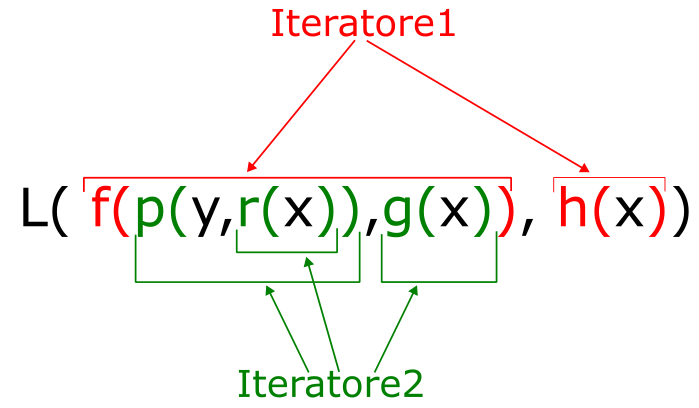
\includegraphics[width=\columnwidth]{figures/literal-iterator.png}
    \caption{Uso degli iteratori per il calcolo della \emph{VarDepth}}
    \label{fig:lit-it}
\end{figure}
In questo caso la prima funzione è iterativa, mentre la seconda è ricorsiva per sfruttare la struttura del letterale.
\begin{algorithm}[H]
    \caption{Prima funzione che scorre i termini esterni del letterale}
    \begin{algorithmic}
        \Function{\textsc{ComputeVarDepth1}}{lit : literal}
        \If{literal \textbf{is} ground}
            \State setLiteralVarDepth(-1, lit)
            \State \underline{\textbf{return}}
        \EndIf
        \State \textbf{var} max, varDepth : int
        \State max = 0
        \ForAll{term \textbf{in} lit} \Comment{Iteratore1 qui scorre i termini esterni}
            \State varDepth = 0
            \State varDepth = 1 + \textsc{ComputeVarDepth2}(term)
            \If{max $<$ varDepth}
                \State max = varDepth
            \EndIf
        \EndFor
        \State setLiteralVarDepth(max, lit)
        \EndFunction
    \end{algorithmic}
\end{algorithm}
Se il letterale è \emph{ground}\footnote{Un letterale è detto \emph{ground} se è privo di variabili}, la \emph{VarDepth} di \emph{lit} viene impostata a $-1$ tramite la funzione 
\emph{setLiteralVarDepth()}.
Nel caso non sia \emph{ground}, allora viene calcolata la massima profondità di ciascun termine esterno tramite la seconda funzione \textsc{ComputeVarDepth2}().
Alla fine il risultato sarà la massima profondità calcolata tra tutti i termini. 
\begin{algorithm}[H]
    \caption{Seconda funzione che scorre i sottotermini in profondità}
    \begin{algorithmic}
        \Function{\textsc{ComputeVarDepth1}}{term : term of literal}
        \State \textbf{var} max, varDepth : int
        \State max = 0
        \ForAll{subterm \textbf{in} term} \Comment{Iteratore2 qui scorre i sottotermini}
            \State varDepth = 0
            \State varDepth = 1 + \textsc{ComputeVarDepth2}(subterm) \Comment{Visita in profondità}
            \If{max $<$ varDepth}
                \State max = varDepth
            \EndIf
        \EndFor
        \State \underline{\textbf{return} max}
        \EndFunction
    \end{algorithmic}
\end{algorithm}
\section{Resolution}
La nuova inferenza implementata, denominata $\prec$-\emph{ordered resolution}, eredita la classe \\\verb|GeneratingInferenceEngine| (figura \ref{fig:genengineclass}), 
 in modo da avere a disposizione tutti i metodi necessari per essere inserita 
nell'algoritmo di saturazione e generare nuove clausole.
La funzione principale di questa classe è \emph{generateClause}() che sfrutta le varie strutture 
dati messe a disposizione da \textsc{Vampire}. 

Il metodo viene eseguito dopo la selezione di una clausola e la conseguente attivazione. La struttura dati fondamentale 
è l'indice che tiene traccia di tutte le clausole e permette di trovarne una da unificare con quella selezionata.
Sia $\{A_1\}\cup R_1$ clausola selezionata, allora il risultato della query sull'indice viene salvato 
in un altra struttura dati che comprende:
\begin{itemize}
    \item una clausola $\{\lnot A_2\}\cup R_2$ candidata a unificare con la clausola selezionata 
    \item un letterale $\{\lnot A_2\}$ candidato all'unificazione con uno dei letterali della clausola selezionata (in questo caso $\{A_1\}$)
\end{itemize} 
\begin{algorithm}[H]
    \caption{Funzione \emph{generateClause}()}
    \begin{algorithmic}
        \State \textbf{var} selectedLiteral, candidateLiteral : literal
        \State \textbf{var} selectedClause, candidateClause, result : clause
        \If{\textsc{IsMaximal}(selectedLiteral, selectedClause) $\land$ \textsc{IsMaximal}(candidateLiteral)}
            \State result = \emph{unify(selectedClause, candidateClause)}
            \State \underline{\textbf{return} result}
        \Else
            \State \underline{\textbf{return} NULL}
        \EndIf
    \end{algorithmic}
\end{algorithm}
Sia $\prec$ un ordinamento definito come prescritto dalla definizione \ref{ord-def}.
La funzione \emph{generateClause}() verifica se il letterale 
$\{A_1\}$ in $\{A_1\}\cup R_1$ e il letterale $\{\lnot A_2\}$ in $\{\lnot A_2\}\cup R_2$ sono massimali 
(secondo l'ordinamento $\prec$) tramite la funzione \textsc{IsMaximal}() .
Nel caso siano massimali, allora viene applicata la \emph{resolution} e l'unificazione tramite la funzione \emph{unify}().
\begin{equation*}
    \begin{gathered}
        \underline{\{\underline{A_1}\} \lor R_1 \quad\{\underline{\lnot A_2}\}\lor R_2}\\
        (R_1 \lor R_2)\theta
    \end{gathered}
\end{equation*}
In caso contrario non viene generata alcuna clausola.
\begin{algorithm}[H]
    \caption{Funzione che controlla se un letterale è il massimale in una clausola}
    \begin{algorithmic}
        \Function{\textsc{IsMaximal}}{maxLit : literal, cl : clause}
            \ForAll{lit \textbf{in} cl}
                \State varDepth = \emph{getVarDepth}(lit)
                \If{(max$<$varDepth) $\land$ (\emph{Var}(lit)$\not\subseteq$\emph{Var}(maxLit))}
                    \State \underline{\textbf{return} $\bot$}
                \EndIf
            \EndFor
            \State \underline{\textbf{return} $\top$}
        \EndFunction
    \end{algorithmic}
\end{algorithm}
Seguendo la definizione \ref{ord-def}, la funzione \textsc{IsMaximal}() controlla se 
un letterale \emph{maxLit} è massimale nella clausola ovvero:
\begin{itemize}
    \item se la \emph{VarDepth} di \emph{maxLit} è maggiore o uguale di tutte le \emph{VarDepth} degli altri letterali nella clausola, o
    \item se l'insieme delle variabili di \emph{maxLit} contiene l'insieme delle variabili degli altri letterali nella clausola
\end{itemize}
La funzione restituisce $\bot$ se entrambe le condizioni non sono rispettate.
\section{Classificazione}\label{class}
A fini sperimentali, viene implementato un classificatore per riconoscere, tra un insieme di problemi casuali,
quali di questi appartengono al frammento \emph{guarded}.
Il classificatore viene richiamato dopo il \emph{parser} di \textsc{Vampire} 
ed è composto da due funzioni principali; una per analizzare le formule arbitrarie della logica del primo ordine e un'altra per analizzare clausole.

La prima funzione sfrutta, come il \emph{preprocessor}, 
la struttura ad albero della formula ed è dunque ricorsiva.
\begin{algorithm}[H]
    \caption{Visita dell'albero della formula parte 1}
    \begin{algorithmic}[1]
        \Function{\textsc{Visit}}{input : formula}
            \Case{connective \textbf{of} input}
                \Switch{$\top,\bot$, Literal}
                    \State \underline{\textbf{return} $\top$}
                \EndSwitch
                \Switch{$\lnot$}
                    \State \underline{\textbf{return} \textsc{Visit}(subformula \textbf{of} input)}
                \EndSwitch
                \Switch{$\rightarrow,\leftrightarrow$}
                    \State \textbf{var} left, right : formula
                    \State left = \textsc{Visit}(left subformula \textbf{of} input)
                    \If{left $=\top$}
                        \State \underline{\textbf{return} \textsc{Visit}(right subformula \textbf{of} input)}
                    \EndIf
                    \State \underline{\textbf{return} $\bot$}
                \EndSwitch
                \Switch{$\land,\lor$}
                    \ForAll{subformula \textbf{in} input}
                        \State subformula = \textsc{Visit}(subformula)
                        \If{subformula $\neq \top$}
                            \State \underline{\textbf{return} $\bot$}
                        \EndIf
                    \EndFor
                    \State \underline{\textbf{return} $\top$} 
                \EndSwitch
                \Switch{$\exists$}
                    \State \textbf{var} subformula : formula
                    \State \textbf{var} vars : sets of bounded variables 
                    \State \textbf{var} lit : literal
                    \State \textbf{var} guardFound : bool
                    \State subformula = subformula \textbf{of} input
                    \State vars = \emph{getBoundedVariables}(input)
                    \If{connective \textbf{of} subformula \textbf{is} $\land$} \label{exists}
                        \State guardFound $=\bot$
                        \While{sub-subformula \textbf{in} subformula $\land$ guardFound $=\bot$}
                            \If{sub-subformula \textbf{is} Literal}
                                \State lit = literal \textbf{of} sub-subformula
                                \If{\emph{isPositive}(lit) $\land$ \emph{isGuard}(lit, vars)} \label{pos-guard}
                                    \State guardFound = $\top$
                                \EndIf
                            \EndIf
                        \EndWhile
                        \If{guardFound $==\top$}
                            \State \underline{\textbf{return} \textsc{Visit}(subformula)} 
                        \Else
                            \State \underline{\textbf{return} $\bot$}
                        \EndIf
                    \Else 
                        \State \underline{\textbf{return} $\bot$}
                    \EndIf
                \EndSwitch
                \algstore{myalg} 
            %\EndCase
        %\EndFunction
    \end{algorithmic}
\end{algorithm}

\begin{algorithm}[H]
    \caption{Visita dell'albero della formula parte 2}
    \begin{algorithmic}[1]
        \algrestore{myalg}
            \Switch{$\forall$}
                \State \textbf{var} subformula : formula
                \State \textbf{var} vars : sets of bounded variables 
                \State \textbf{var} lit : literal
                \State \textbf{var} guardFound : bool
                \State subformula = \emph{getSubformula}(input)
                \State vars = \emph{getBoundedVariables}(input)
                \State left = \emph{getLeft}(subformula)
                \If{(connective \textbf{of} subformula \textbf{is} $\rightarrow$) $\land$ (left \textbf{is} Literal)} \label{forall-imp}
                    \State lit = literal \textbf{of} left
                    \If{\emph{isPositive}(lit) $\land$ \emph{isGuard}(lit, vars)} \label{pos-guard-for}
                        \State \underline{\textbf{return} \textsc{Visit}(right subformula \textbf{of} subformula)} 
                    \Else
                        \State \underline{\textbf{return} $\bot$}
                    \EndIf
                \ElsIf{connective \textbf{of} subformula \textbf{is} $\lor$} \label{forall-or}
                    \State guardFound = $\bot$
                    \While{subformula \textbf{in} input $\land$ guardFound $=\bot$}
                        \If{subformula \textbf{is} Literal}
                            \State lit = literal \textbf{of} subformula
                            \If{\emph{isNegative}(lit) $\land$ \emph{isGuard}(lit, vars)} \label{neg-guard}
                                \State guardFound = $\top$
                            \EndIf
                        \EndIf
                    \EndWhile
                    \If{guardFound $=\top$}
                        \State \underline{\textbf{return} \textsc{Visit}(subformula)} 
                    \Else
                        \State \underline{\textbf{return} $\bot$}
                    \EndIf
                \EndIf
                \State \underline{\textbf{return} $\bot$}
            \EndSwitch 
        \EndCase
        \EndFunction
    \end{algorithmic}
\end{algorithm}
Durante la visita l'algoritmo controlla se nell'intero albero sono presenti formule del tipo: 
\begin{itemize}
    \item $\forall\bar{x}(a \rightarrow A)$ (riga \ref{forall-imp}), 
    \item $\forall\bar{x}(a \lor A)$ (riga \ref{forall-or}),
    \item $\exists\bar{x}(a \land A)$ (riga \ref{exists})
\end{itemize}
Nel primo caso verifica che $a$ sia un letterale positivo e una guardia tramite
 le funzioni \emph{isPositive}() e \emph{isGuard}() (riga \ref{pos-guard-for}). 
Nel secondo e nell'ultimo caso si scorrono tutte le sottoformule per trovare, rispettivamente, 
una guardia negativa (riga \ref{neg-guard}) e una guardia positiva (riga \ref{pos-guard}).
\begin{algorithm}
    \caption{Funzione che verifica se un letterale è una guardia}
    \begin{algorithmic}
        \Function{\textsc{IsGuard}}{lit : literal, vars : sets of variables}
            \State \textbf{var} literalVars : sets of variables
            \State literalVars = getVariablesOf(lit)
            \ForAll{variable \textbf{in} vars}
                \State \textbf{var} foundVariable = $\bot$
                \While{litVar \textbf{in} literalVars $\land$ foundVariable $==\bot$}
                    \If{litVar $==$ variable}
                        \State foundVariable = $\top$
                    \EndIf
                \EndWhile
                \If{foundVariable $==\bot$}
                    \State \underline{\textbf{return} $\bot$}
                \EndIf
            \EndFor
            \State \underline{\textbf{return} $\top$}
        \EndFunction
    \end{algorithmic}
\end{algorithm}

La funzione \textsc{IsGuard}() verifica se un letterale è una guardia, ovvero se contiene 
almeno una volta le variabili libere \emph{vars} delle altre sottoformule. 

\begin{algorithm}[H]
    \caption{Funzione che verifica se una clausola è \emph{guarded}}
    \begin{algorithmic}
        \State \textbf{var} cl : clause
        \State \textbf{var} vars : clause variables set
        \State \textbf{var} checkGuard : bool
        \State checkGuard = $\bot$
        \ForAll{lit \textbf{in} cl}
            \If{\emph{isNegative(lit)} $\land$ foundVariable $==\bot$}\label{cl-guard-neg}
                \State checkGuard = \textsc{IsGuard}(lit, vars)
                \If{checkGuard $==\top$}
                    \State \textbf{continue}
                \EndIf
            \EndIf
            \ForAll{term \textbf{in} lit} \label{term-1}
                \If{$\lnot$\emph{containsAllVariablesOfClause}(term,vars)} \label{term-2}
                    \State \underline{\textbf{return} $\bot$}
                \EndIf
            \EndFor
        \EndFor
        \State \underline{\textbf{return} checkGuard}
    \end{algorithmic}
\end{algorithm}
La seconda funzione che analizza le clausole verifica se esiste una guardia negativa (riga \ref{cl-guard-neg}), 
tramite la funzione \textsc{IsGuard}(), e se i termini funzionali non ground contengono 
tutte le variabili della clausola (righe \ref{term-1}, \ref{term-2}).




    \clearpage
    \chapter{Risultati sperimentali}\label{third-c}
In questo capitolo vengono presentati i risultati sperimentali del confronto 
tra \textsc{Vampire} originale e \textsc{Vampire} con la nuova procedura di decisione.

Per gli esperimenti sono stati utilizzati i problemi della libreria TPTP versione 8.2.0 \cite{Sut17}.
I problemi presi in esame sono privi di uguaglianza, poiché la procedura di decisione 
analizzata in questa tesi tratta 
solo questo tipo di problemi. 
\'E possibile dividere i problemi in due insiemi:
uno comprende quelli composti da formule della logica del primo ordine (FOF), mentre l'altro 
comprende i problemi composti da clausole (CNF).
\begin{table}[H]
    \begin{center}
    \caption{Numero di problemi}
    \begin{tabular}{ccc}
        \toprule % <-- Toprule here
        &\textbf{FOF} & \textbf{CNF}\\
        \midrule % <-- Midrule here
        Senza equality & 1969 & 2274\\
        \bottomrule % <-- Bottomrule here
        \textbf{\emph{Guarded}} & \textbf{52} & \textbf{62}\\
    \end{tabular}
    \label{tab:prob}
\end{center}
\end{table} 
Entrambi gli insiemi sono stati dati in input 
al classificatore (capitolo \ref{class}) e il risultato è quello riportato in tabella \ref{tab:prob}:
52 problemi di tipo FOF su 1969 e 62 problemi di tipo CNF su 2274 sono \emph{guarded}
(7 di questi 52 problemi di tipo FOF non vengono presi in considerazione nei grafici seguenti, in quanto 
non possono essere risolti nel tempo limite stabilito). Di seguito viene fornita una numerazione 
dei problemi FOF e CNF in modo da rendere più chiara la lettura dei grafici.
\noindent\begin{table}[H]
    \caption{Numerazione dei problemi FOF}
    \resizebox{\linewidth}{!}{
        \begin{tabular}{cccccc}
            \csvautotabular{data/problem.csv} &
            \csvautotabular{data/problem2.csv} &
            \csvautotabular{data/problem3.csv}
        \end{tabular}}
        
\end{table}
\begin{table}[H]
    \caption{Numerazione dei problemi CNF}
    \resizebox{\linewidth}{!}{
        \begin{tabular}{cccccccc}
            \csvautotabular{data/problem-cnf.csv} &
            \csvautotabular{data/problem-cnf2.csv} &
            \csvautotabular{data/problem-cnf3.csv} & 
            \csvautotabular{data/problem-cnf4.csv} 
        \end{tabular}}
        
\end{table}
Nei test, \textsc{Vampire} con la nuova procedura di decisione è indicato con \textsc{Guarded}.
I primi test sono stati eseguiti con le seguenti opzioni di \textsc{Vampire}:
\begin{center}
    \verb|--sa otter -t 10m -m 8000|    
\end{center}
L'algoritmo di saturazione scelto è \emph{otter}, il tempo massimo di timeout è 10 minuti 
e il limite massimo di memoria occupabile è 8000 Mb.
\section{Problemi FOF}
\begin{figure}[H]
    \centering
    \begin{tikzpicture}
        \begin{axis}[
            width=\textwidth,
            xlabel={Problema},
            ylabel={Tempo (s)},
            legend style={at={(0.5,1)},       
            anchor=north,legend columns=-1},
            xtick=data,
            axis x line=bottom,     
            axis y line=left,
            xmajorgrids=true,     
            grid style=dashed,
            xtick align=outside,
            x tick label style = {
                %yshift={-mod(\ticknum,2)*0.1cm}, 
                font = \small, rotate=70, align = center},
        ]
        \legend{\textsc{Vampire}, \textsc{Guarded}}
        \addplot[color=red]table{data/1-vampire-time.dat};
        \addplot[color=blue]table{data/1-guarded-time.dat};
        \end{axis}
    \end{tikzpicture}
    \caption{Tempo impiegato da \textsc{Vampire} e \textsc{Guarded} per risolvere problemi FOF}
\end{figure}
Dai primi test sui problemi FOF emerge che, nella maggior parte dei problemi, \textsc{Guarded} è efficiente
tanto quanto \textsc{Vampire} in termini di tempo. La differenza tra i due, essendo nell'ordine dei millisecondi,
non è significativa. 
Ci sono alcune eccezioni: i problemi MED011+1 (n.5) e NLP263+1 (n.6) sono a favore di
\textsc{Vampire} rispettivamente di circa 10 e 18 secondi, mentre il problema SYO525+1.018 (n.45) è a favore di \textsc{Guarded} di circa 12 secondi.

\begin{figure}[H]
    \begin{tikzpicture}
        \begin{axis}[
            width=\textwidth,
            xlabel={Problema},
            ylabel={Memoria (Kb)},
            legend style={at={(0.5,1)},       
            anchor=north,legend columns=-1},
            every y tick scale label/.style={
                at={(0.07,1)},anchor=north east,inner sep=0pt},
            xtick=data,
            axis x line=bottom,     
            axis y line=left,
            xmajorgrids=true,     
            grid style=dashed,
            xtick align=outside,
            x tick label style = {
                %yshift={-mod(\ticknum,2)*0.1cm}, 
                font = \small, rotate=70, align = center},
        ]
        \legend{\textsc{Vampire}, \textsc{Guarded}}
        \addplot[color=red]table{data/1-vampire-mem.dat};
        \addplot[color=blue]table{data/1-guarded-mem.dat};
        \end{axis}
    \end{tikzpicture}
    \caption{Memoria occupata da \textsc{Vampire} e \textsc{Guarded} per risolvere problemi FOF}
\end{figure}

\textsc{Vampire} e \textsc{Guarded} sono molto simili anche in termini di memoria occupata per la risoluzione di un problema.
L' unica eccezione rilevante 
è il problema NLP263+1 (n.6) in cui \textsc{Guarded} occupa $6.7\times10^5$ Kb di memoria, mentre \textsc{Vampire} solo $5.2\times10^5$ Kb.\\\\
Alla fine di questa batteria di test, l'analisi ha posto particolare attenzione alle eccezioni. 
\begin{description}
    \item[Memoria:] La tendenza di \textsc{Guarded} ad occupare più memoria in alcuni problemi proseguirà anche nei prossimi test
    poiché, in problemi complessi e di grandi dimensioni, la trasformazione strutturale 
    $\text{\emph{Struct}}_\forall$ aggiunge nuove formule del tipo $\forall\bar{x}\bar{y}(\lnot a \lor \lnot\alpha \lor A)$ 
    quindi occupa molto più spazio rispetto a \textsc{Vampire}.
    \item[Tempo:] Nelle eccezioni in cui \textsc{Vampire} impiega meno tempo, è utilizzata
    una tecnica di \emph{preprocessing} detta \emph{unused predicate definition removal}.
    Una definizione di un predicato è una formula del tipo 
    \[\forall(X_1,\dots,X_n) : p(X_1, \dots, X_n) \leftrightarrow F\]
    in cui $p$ predicato non risulta in $F$. 
    Con questa tecnica \textsc{Vampire} si può comportare in 3 modi:
    \begin{enumerate}
        \item se $p$ è presente nel resto del problema solo in forma positiva, allora $\leftrightarrow$ della definizione
        viene sostituito da $\rightarrow$;
        \item se $p$ non è presente nel resto del problema, allora la definizione può essere eliminata;
        \item altrimenti la definizione non viene modificata
    \end{enumerate}
    In tal modo \textsc{Vampire} riesce a risolvere i problemi FOF in modo più rapido.
\end{description}

Nei prossimi test, la tecnica di \emph{unused predicate definition removal} (updr) 
verrà disattivata da \textsc{Vampire}. Infatti, le opzioni saranno:
\begin{center}
    \verb|-updr off --sa otter -t 10m -m 8000|    
\end{center}

\begin{figure}[H]
    \begin{tikzpicture}
        \begin{axis}[
            width=\textwidth,
            xlabel={Problema},
            title style={align=center},
            ylabel={Tempo (s)},
            legend style={at={(0.5,1)},       
            anchor=north,legend columns=-1},
            xtick=data,
            axis x line=bottom,     
            axis y line=left,
            xmajorgrids=true,     
            grid style=dashed,
            xtick align=outside,
            x tick label style = {
                %yshift={-mod(\ticknum,2)*0.1cm}, 
                font = \small, rotate=70, align = center},
        ]
        \legend{\textsc{Vampire}, \textsc{Guarded}}
        \addplot[color=red]table{data/2-vampire-time.dat};
        \addplot[color=blue]table{data/2-guarded-time.dat};
        \end{axis}
    \end{tikzpicture}
    \caption{Tempo impiegato da \textsc{Vampire} e \textsc{Guarded} per risolvere problemi FOF con \emph{updr} disattivata}
\end{figure}

Con la disattivazione della \emph{updr}, le prestazioni di \textsc{Vampire} peggiorano significativamente. 
Infatti, in questo modo \textsc{Vampire} impiega più tempo di \textsc{Guarded}, con una 
differenza di circa 10 secondi nel problema MED011+1 (n.5) e di circa 20 secondi in NLP263+1 (n.6). In questi test \textsc{Vampire}
impiega circa 20 secondi in più nel problema MED011+1 (n.5) e circa 38 secondi in più nel problema NLP263+1 (n.6) rispetto alla batteria di 
test precedente.\\\\
\begin{figure}[H]
    \begin{tikzpicture}
        \begin{axis}[
            width=\textwidth,
            title style={align=center},
            xlabel={Problema},
            ylabel={Memoria (Kb)},
            legend style={at={(0.5,1)},       
            anchor=north,legend columns=-1},
            every y tick scale label/.style={
                at={(0.07,1)},anchor=north east,inner sep=0pt},
            xtick=data,
            axis x line=bottom,     
            axis y line=left,
            xmajorgrids=true,     
            grid style=dashed,
            xtick align=outside,
            x tick label style = {
                %yshift={-mod(\ticknum,2)*0.1cm}, 
                font = \small, rotate=70, align = center},
        ]
        \legend{\textsc{Vampire}, \textsc{Guarded}}
        \addplot[color=red]table{data/2-vampire-mem.dat};
        \addplot[color=blue]table{data/2-guarded-mem.dat};
        \end{axis}
    \end{tikzpicture}
    \caption{Memoria occupata da \textsc{Vampire} e \textsc{Guarded} per risolvere problemi FOF con \emph{updr} disattivata}
\end{figure}


Disattivando l'\emph{updr}, la quantità di memoria occupata da \textsc{Vampire} per il problema NLP263+1 aumenta al punto 
da superare quella utilizzata da \textsc{Guarded}. Nonostante ciò, la differenza non è da considerare significativa.

\section{Problemi CNF}
\begin{figure}[H]
    \begin{tikzpicture}
        \begin{axis}[
            width=\textwidth,
            xlabel={Problema},
            ylabel={Tempo (s)},
            legend style={at={(0.7,1)},       
            anchor=north,legend columns=-1},
            xtick=data,
            axis x line=bottom,     
            axis y line=left,
            xmajorgrids=true,     
            grid style=dashed,
            xtick align=outside,
            x tick label style = {
                yshift={-mod(\ticknum,2)*0.35cm}, 
                font = \small, rotate=90, align = center},
        ]
        \legend{\textsc{Vampire}, \textsc{Guarded}}
        \addplot[color=red]table{data/1-cnf-vampire-time.dat};
        \addplot[color=blue]table{data/1-cnf-guarded-time.dat};
        \end{axis}
    \end{tikzpicture}
    \caption{Tempo impiegato da \textsc{Vampire} e \textsc{Guarded} per risolvere problemi CNF}
\end{figure}


Dai test sui problemi CNF emergono gli stessi risultati dei precedenti test sui problemi FOF: nella maggior parte dei problemi, \textsc{Guarded} è efficiente
quanto \textsc{Vampire}, sia in termini di tempo che di memoria. In questo caso, la differenza è ancora minore rispetto ai problemi FOF.
L'unica eccezione è il problema PUZ036-1.005 (n.25) in cui \textsc{Vampire} impiega circa 0,2 secondi e occupa 1100 Kb, mentre \textsc{Guarded}
circa 4 secondi e 15000 Kb.

\begin{figure}[H]
    \begin{tikzpicture}
        \begin{axis}[
            width=\textwidth,
            xlabel={Problema},
            ylabel={Memoria (Kb)},
            legend style={at={(0.7,1)},       
            anchor=north,legend columns=-1},
            every y tick scale label/.style={
                at={(0.07,1)},anchor=north east,inner sep=0pt},
            xtick=data,
            axis x line=bottom,     
            axis y line=left,
            xmajorgrids=true,     
            grid style=dashed,
            xtick align=outside,
            x tick label style = {
                yshift={-mod(\ticknum,2)*0.35cm}, 
                font = \small, rotate=70, align = center},
        ]
        \legend{\textsc{Vampire}, \textsc{Guarded}}
        \addplot[color=red]table{data/1-cnf-vampire-mem.dat};
        \addplot[color=blue]table{data/1-cnf-guarded-mem.dat};
        \end{axis}
    \end{tikzpicture}
    \caption{Memoria occupata da \textsc{Vampire} e \textsc{Guarded} per risolvere problemi CNF}
\end{figure}

Alla fine di questi primi test sui problemi CNF, è stata effettuata l'analisi sul problema PUZ036-1.005 (n.25).
\textsc{Vampire}, nell'algoritmo di saturazione, utilizza la \emph{forward subsumption},
un'inferenza che fa parte delle \emph{forward simplification} (capitolo \ref{sec-kernel}) utile per eliminare le ridondanze.
Questa tecnica permette a \textsc{Vampire} di essere più veloce ed efficiente.

Nei prossima batteria di test, la tecnica di \emph{forward subsumption} (fs) verrà disattivata da \textsc{Vampire} 
infatti le opzioni saranno:
\begin{center}
    \verb|-fs off --sa otter -t 10m -m 8000|    
\end{center}
Si noti che i test sono stati effettuati anche con \emph{updr} disattivata, ma
non stati riportati i risultati poiché non c'è stato nessun cambiamento significativo dei valori. Lo stesso 
vale anche per l'opzione \emph{fs} nei problemi FOF. Infatti, su questi problemi, sono stati 
eseguiti i test anche con \emph{fs} disattivata ma i risultati non hanno portato a nessun cambiamento rilevante.

\begin{figure}[H]
    \begin{tikzpicture}
        \begin{axis}[
            width=\textwidth,
            xlabel={Problema},
            title style={align=center},
            ylabel={Tempo (s)},
            legend style={at={(0.7,1)},       
            anchor=north,legend columns=-1},
            xtick=data,
            axis x line=bottom,     
            axis y line=left,
            xmajorgrids=true,     
            grid style=dashed,
            xtick align=outside,
            x tick label style = {
                yshift={-mod(\ticknum,2)*0.35cm}, 
                font = \small, rotate=90, align = center},
        ]
        \legend{\textsc{Vampire}, \textsc{Guarded}}
        \addplot[color=red]table{data/3-cnf-vampire-time.dat};
        \addplot[color=blue]table{data/3-cnf-guarded-time.dat};
        \end{axis}
    \end{tikzpicture}
    \caption{Tempo impiegato da \textsc{Vampire} e \textsc{Guarded} per risolvere problemi CNF con \emph{forward subsumption} disattivata per entrambi}
\end{figure}

Con la disattivazione della \emph{forward subsumption}, \textsc{Vampire} peggiora sia in termini 
di tempo che di memoria occupata nel problema PUZ036-1.005 (n.25). La differenza di tempo tra \textsc{Vampire}
e \textsc{Guarded} si assottiglia molto in questo problema, infatti è di circa mezzo secondo.

\begin{figure}[H]
    \begin{tikzpicture}
        \begin{axis}[
            width=\textwidth,
            xlabel={Problema},
            title style={align=center},
            ylabel={Memoria (Kb)},
            legend style={at={(0.7,1)},       
            anchor=north,legend columns=-1},
            every y tick scale label/.style={
                at={(0.07,1)},anchor=north east,inner sep=0pt},
            xtick=data,
            axis x line=bottom,     
            axis y line=left,
            xmajorgrids=true,     
            grid style=dashed,
            xtick align=outside,
            x tick label style = {
                yshift={-mod(\ticknum,2)*0.35cm}, 
                font = \small, rotate=90, align = center},
        ]
        \legend{\textsc{Vampire}, \textsc{Guarded}}
        \addplot[color=red]table{data/3-cnf-vampire-mem.dat};
        \addplot[color=blue]table{data/3-cnf-guarded-mem.dat};
        \end{axis}
    \end{tikzpicture}
    \caption{Memoria occupata da \textsc{Vampire} e \textsc{Guarded} \\per risolvere problemi CNF con \emph{forward subsumption} disattivata per entrambi}
\end{figure}

Con la disattivazione della \emph{forward subsumption}, \textsc{Vampire} e \textsc{Guarded} occupano  
circa la stessa quantità di memoria.
\clearpage


    %other chapters here..

    \chapter{Conclusioni}\label{fourth-c}
In conclusione, quello che è emerso dal capitolo \ref{third-c} è che 
\textsc{Vampire} originale e \textsc{Vampire} esteso con la nuova procedura di decisione sono indistinguibili,
con un'attenzione però alle potenzialità della procedura nei problemi più complessi. 
\'E importante sottolineare che il benchmark effettuato 
è poco significativo, in quanto sono stati selezionati problemi senza uguaglianza, di cui solo
pochi fanno parte del frammento \emph{guarded}.\\\\
Sarebbe possibile approfondire l'analisi della procedura di decisione tramite la generazione di problemi complessi che fanno 
parte della logica modale. 

Inoltre, grazie al classificatore (cap \ref{class}), si è osservato che circa 640 problemi in cui è presente l'uguaglianza sono \emph{guarded}. 
Quindi, un'ulteriore indagine può essere condotta sullo studio di \citeauthor{ganzinger1999superposition}, con l'implementazione della 
procedura di decisione basata sulla \emph{superposition} \cite{ganzinger1999superposition}. In questo modo, sarebbe possibile 
includere nell'analisi quei problemi \emph{guarded} in cui è presente l'uguaglianza. 

    %\input{_chapters/4-appendix.tex}
    
   
    \newpage\pagestyle{backmatter}
    \printbibliography[heading=bibintoc]

    %\listoffigures
 
    %\listoftables

\end{document}